\documentclass[mathserif,compress]{beamer}\usepackage{graphicx, color}
%% maxwidth is the original width if it is less than linewidth
%% otherwise use linewidth (to make sure the graphics do not exceed the margin)
\makeatletter
\def\maxwidth{ %
  \ifdim\Gin@nat@width>\linewidth
    \linewidth
  \else
    \Gin@nat@width
  \fi
}
\makeatother

\definecolor{fgcolor}{rgb}{0.2, 0.2, 0.2}
\newcommand{\hlnumber}[1]{\textcolor[rgb]{0,0,0}{#1}}%
\newcommand{\hlfunctioncall}[1]{\textcolor[rgb]{0.501960784313725,0,0.329411764705882}{\textbf{#1}}}%
\newcommand{\hlstring}[1]{\textcolor[rgb]{0.6,0.6,1}{#1}}%
\newcommand{\hlkeyword}[1]{\textcolor[rgb]{0,0,0}{\textbf{#1}}}%
\newcommand{\hlargument}[1]{\textcolor[rgb]{0.690196078431373,0.250980392156863,0.0196078431372549}{#1}}%
\newcommand{\hlcomment}[1]{\textcolor[rgb]{0.180392156862745,0.6,0.341176470588235}{#1}}%
\newcommand{\hlroxygencomment}[1]{\textcolor[rgb]{0.43921568627451,0.47843137254902,0.701960784313725}{#1}}%
\newcommand{\hlformalargs}[1]{\textcolor[rgb]{0.690196078431373,0.250980392156863,0.0196078431372549}{#1}}%
\newcommand{\hleqformalargs}[1]{\textcolor[rgb]{0.690196078431373,0.250980392156863,0.0196078431372549}{#1}}%
\newcommand{\hlassignement}[1]{\textcolor[rgb]{0,0,0}{\textbf{#1}}}%
\newcommand{\hlpackage}[1]{\textcolor[rgb]{0.588235294117647,0.709803921568627,0.145098039215686}{#1}}%
\newcommand{\hlslot}[1]{\textit{#1}}%
\newcommand{\hlsymbol}[1]{\textcolor[rgb]{0,0,0}{#1}}%
\newcommand{\hlprompt}[1]{\textcolor[rgb]{0.2,0.2,0.2}{#1}}%

\usepackage{framed}
\makeatletter
\newenvironment{kframe}{%
 \def\at@end@of@kframe{}%
 \ifinner\ifhmode%
  \def\at@end@of@kframe{\end{minipage}}%
  \begin{minipage}{\columnwidth}%
 \fi\fi%
 \def\FrameCommand##1{\hskip\@totalleftmargin \hskip-\fboxsep
 \colorbox{shadecolor}{##1}\hskip-\fboxsep
     % There is no \\@totalrightmargin, so:
     \hskip-\linewidth \hskip-\@totalleftmargin \hskip\columnwidth}%
 \MakeFramed {\advance\hsize-\width
   \@totalleftmargin\z@ \linewidth\hsize
   \@setminipage}}%
 {\par\unskip\endMakeFramed%
 \at@end@of@kframe}
\makeatother

\definecolor{shadecolor}{rgb}{.97, .97, .97}
\definecolor{messagecolor}{rgb}{0, 0, 0}
\definecolor{warningcolor}{rgb}{1, 0, 1}
\definecolor{errorcolor}{rgb}{1, 0, 0}
\newenvironment{knitrout}{}{} % an empty environment to be redefined in TeX

\usepackage{alltt} 
\usepackage{beamerthemeDresden} 
\usepackage[english]{babel}
\usepackage{amsmath,amssymb}
\usepackage[latin1]{inputenc}
\usepackage{palatino}
\usepackage{graphicx}
\usepackage{subfigure}
\usepackage{pgf}
\usepackage{relsize}
\def\beq{\begin{equation}}
\def\eeq{\end{equation}}
\def\bit{\begin{itemize}}
\def\eit{\end{itemize}}
\def\bdm{\begin{displaymath}}
\def\edm{\end{displaymath}}
\def\ben{\begin{enumerate}}
\def\een{\end{enumerate}}
\def\bb{\mathbf{b}}
\def\bc{\mathbf{c}}
\def\bd{\mathbf{d}}
\def\bh{\mathbf{h}}
\def\bm{\mathbf{m}}
\def\br{\mathbf{r}}
\def\bs{\mathbf{s}}
\def\bu{\mathbf{u}}
\def\bv{\mathbf{v}}
\def\bw{\mathbf{w}}
\def\bx{\mathbf{x}}
\def\by{\mathbf{y}}
\def\bz{\mathbf{z}}
\def\bA{\mathbf{A}}
\def\bD{\mathbf{D}}
\def\bG{\mathbf{G}}
\def\bI{\mathbf{I}}
\def\bQ{\mathbf{Q}}
\def\bR{\mathbf{R}}
\def\bS{\mathbf{S}}
\def\bV{\mathbf{V}}
\def\bW{\mathbf{W}}
\def\bX{\mathbf{X}}
\def\bY{\mathbf{Y}}
\def\bZ{\mathbf{Z}}
\def\cB{\mathcal{B}}
\def\cF{\mathcal{F}}
\def\cI{\mathcal{I}}
\def\cK{\mathcal{K}}
\def\cU{\mathcal{U}}
\def\bbeta{\mbox{\boldmath $\beta$}}
\def\bepsilon{\mbox{\boldmath $\epsilon$}}
\def\bdelta{\mbox{\boldmath $\delta$}}
\def\bgamma{\mbox{\boldmath $\gamma$}}
\def\bldeta{\mbox{\boldmath $\eta$}}
\def\bphi{\mbox{\boldmath $\phi$}}
\def\bkappa{\mbox{\boldmath $\kappa$}}
\def\blambda{\mbox{\boldmath $\lambda$}}
\def\bmu{\mbox{\boldmath $\mu$}}
\def\bnu{\mbox{\boldmath $\nu$}}
\def\btheta{\mbox{\boldmath $\theta$}}
\def\brho{\mbox{\boldmath $\rho$}}
\def\bDelta{\mbox{\boldmath $\Delta$}}
\def\bLambda{\mbox{\boldmath $\Lambda$}}
\def\bSigma{\mbox{\boldmath $\Sigma$}}
\def\var{\textrm{var}}
\def\cov{\textrm{cov}}
\def\log{\textrm{log}}
\def\median{\textrm{median}}
\def\argmin{\textrm{arg min }}
\def\bzero{\mathbf{0}}
\def\bone{\mathbf{1}}
\def\Poi{\textrm{Poi}}
\def\Unif{\textrm{Unif}}
\def\upp{^\prime}
\def\upi{^{-1}}
\newcommand{\cye}[1]{\color{yellow!70!black}#1}
\newcommand{\cre}[1]{\color{red!70!black}#1}
\newcommand{\cbl}[1]{\color{blue!70!black}#1}
\newcommand{\cgr}[1]{\color{green!70!black}#1}
\IfFileExists{upquote.sty}{\usepackage{upquote}}{}
\begin{document}



\title[]{Block Prediction for a Finite Grid}

\author[Jay M. Ver Hoef]{Jay Ver Hoef} 

\institute[NOAA National Marine Mammal Lab]
{
	\normalsize National Marine Mammal Lab \\
	NOAA Fisheries \\
	International Arctic Research Center \\
	Fairbanks, Alaska, USA\\
	\vspace{0.1cm}
}
\date[05/17/13]{}
 
\maketitle
 
% very important to use option [fragile] for frames containing code output!
   
%-------------------------------------------------------------------------------
%                        Introduction
%-------------------------------------------------------------------------------

\section{Introduction}
\subsection{}
\begin{frame}[fragile]
\frametitle{Introduction}
	
	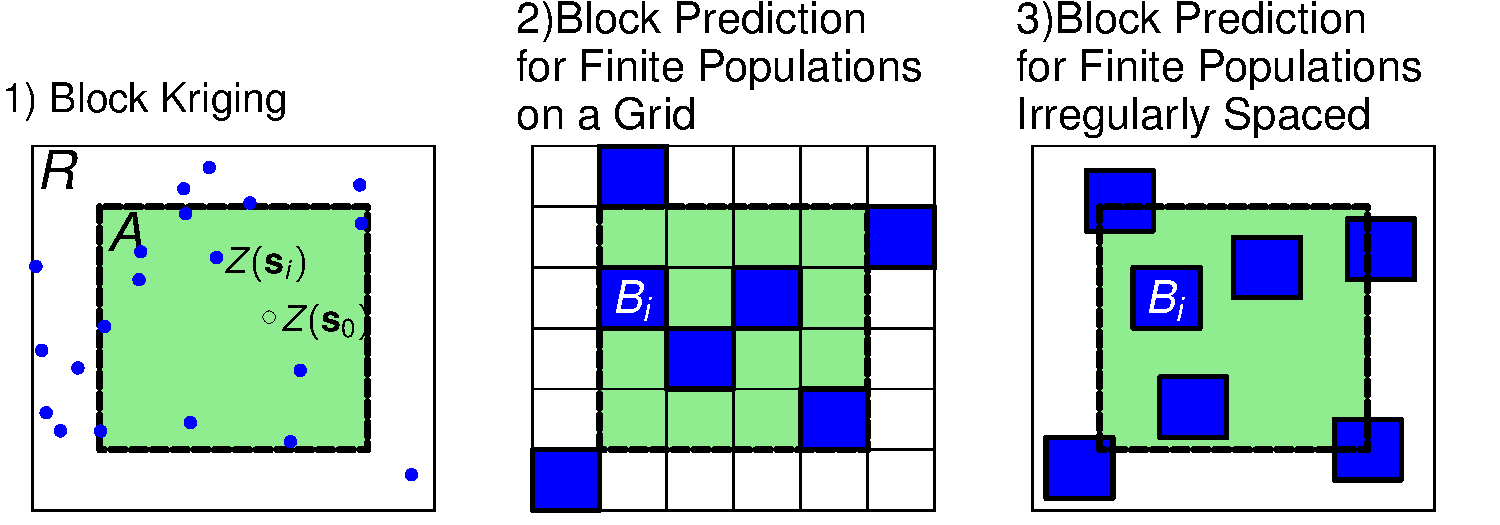
\includegraphics[width=\maxwidth]{figure/Introductory-plot}

\vspace{.5cm}
\scriptsize
Ver Hoef, J.M.  2001.  Predicting finite populations from spatially correlated data. {\it 2000 Proceedings of the Section on Statistics and the Environment of the American Statistical Association}, pgs. 93 - 98. \\

Ver Hoef, J.M.   2008.  Spatial methods for plot-based sampling of wildlife populations.  {\it Environmental and Ecological Statistics} {\bf 15}: 3 - 13.

\end{frame}

%-------------------------------------------------------------------------------
%                 Review of BLUP and Point Prediction
%-------------------------------------------------------------------------------

\section{Theory}
\subsection{}
\begin{frame}[fragile]
\frametitle{Review of BLUP and Point Prediction}
	\vspace{-.5cm}
	\[
		\left(\begin{array}{c}
		\bz \\ Z(\bs_0)
		\end{array}\right)	=
		\left(\begin{array}{c}
		\bX \\ \bx(\bs_0)\upp
		\end{array}\right)\bbeta +
		\left(\begin{array}{c}
		\bepsilon \\ \epsilon(\bs_0)
		\end{array}\right)
	\] \\
	\[ 
		\cov\left(\begin{array}{c}
		\bepsilon \\ \epsilon(\bs_0)
		\end{array}\right) = 
		\left(\begin{array}{cc}
		\bSigma & \bc \\ \bc\upp & \sigma_0^2
		\end{array}\right)
	\]
	 \\
	Best Linear Unbiased Prediction (BLUP) (or [Universal] Kriging) \\
	minimize: $\cre{E(\blambda\upp\bz - Z(\bs_0))^2}$ subject to 	$\cre{E[\blambda\upp\bz] = E[Z(\bs_0)]}  \ \forall \ \bbeta$. \\
	Unbiasedness $\Rightarrow \bX\upp\blambda = \bx(\bs_0)$ \\		
	Minimization yields the solution to:
	\[
		\left(\begin{array}{cc}
		\bSigma & \bX \\ \bX\upp & \bzero
		\end{array}\right)
		\left(\begin{array}{c}
		\blambda \\ \bm
		\end{array}\right) =
		\left(\begin{array}{c}
		\bc \\ \bx(\bs_0)
		\end{array}\right)
	\]
	 

\end{frame}

%-------------------------------------------------------------------------------
%                 BLUP for Finite Populations
%-------------------------------------------------------------------------------

\begin{frame}[fragile]
\frametitle{BLUP for Finite Populations}
	\vspace{-.5cm}
	\[
		\left(\begin{array}{c}
		\bz_s \\ \bz_u
		\end{array}\right)	=
		\left(\begin{array}{c}
		\bX_s \\ \bX_u
		\end{array}\right)\bbeta +
		\left(\begin{array}{c}
		\bepsilon_s \\ \bepsilon_u
		\end{array}\right)
	\] \\
	\[ 
		\cov\left(\begin{array}{c}
		\bepsilon_s \\ \bepsilon_u
		\end{array}\right) = 
		\left(\begin{array}{cc}
		\bSigma_{s,s} & \bSigma_{s,u} \\ \bSigma_{s,u}\upp & \bSigma_{s,s}
		\end{array}\right)
	\]
	 \\
	Best Linear Unbiased Prediction (BLUP) (or [Universal] Kriging) \\
	minimize: $\cre{E(\blambda\upp\bz_s - \bb\upp\bz)^2}$ subject to 	$\cre{E[\blambda\upp\bz_s] = E[\bb\upp\bz] \ \forall \ \bbeta}$. \\
	Unbiasedness $\Rightarrow \bX_s\upp\blambda = \bX_s\upp\bb_s + \bX_u\upp\bb_u $ \\		
	Minimization yields the solution to:
	\[
		\left(\begin{array}{cc}
		\bSigma_{s,s} & \bX_s \\ \bX_s\upp & \bzero
		\end{array}\right)
		\left(\begin{array}{c}
		\blambda \\ \bm
		\end{array}\right) =
		\left(\begin{array}{cc}
		\bSigma_{s,s} & \bSigma_{u,u} \\ \bX_s\upp & \bX_u\upp
		\end{array}\right)
		\left(\begin{array}{c}
		\bb_s  \\ \bb_u & 
		\end{array}\right)
	\]
	 

\end{frame}

%-------------------------------------------------------------------------------
%                 BLUP for Finite Populations
%-------------------------------------------------------------------------------

\begin{frame}[fragile]
\frametitle{BLUP for Finite Populations}

	\begin{center}
		 $\blambda\upp\bz = \bb_s\upp\bz_s + \bb_u\hat{\bz}_u$
	\end{center} \\
	where \\
	\begin{center}
		$\hat{\bz}_u = \bSigma_{u,s}\bSigma\upi_{s,s}(\bz_s - \hat{\bmu}_s) + \hat{\bmu}_u,$
	\end{center} \\
	\begin{center}
		$\hat{\bmu}_u = \bX_u\hat{\bbeta}_{GLS}, \quad \hat{\bmu}_s = \bX_s\hat{\bbeta}_{GLS}, \quad 
\hat{\bbeta}_{GLS} = (\bX_s\upp\bSigma_{s,s}\upi\bX_s)\upi\bX_s\upp\bSigma_{s,s}\upi\bz_s$
	\end{center} \\
	and
	\begin{center}
		 $E(\blambda\upp\bz_s - \bb\bz)^2 = \bb\upp\bSigma\bb - \bc_\bb\upp\bSigma_{s,s}\upi\bc_\bb + \bd_\bb\upp(\bX_s\upp\bSigma_{s,s}\upi\bX_s)\upi\bd_\bb$
	\end{center} \\
	where \\
	\begin{center}
		$\bc_\bb = \bSigma_{s,s}\bb_s + \bSigma_{s,u}\bb_u, \quad \bd_\bb = \bX\upp\bb - \bX_s\upp\bSigma_{s,s}\upi\bc_\bb$
	\end{center} 


\end{frame}

%-------------------------------------------------------------------------------
%                 BLUP for Finite Populations
%-------------------------------------------------------------------------------

\section{Connections}
\subsection{}
\begin{frame}[fragile]
\frametitle{Connections to Sampling Theory}

Let \\
	\begin{array}{ccc}
		\bX = \left(\begin{array}{c}
		\bone_n  \\ \bone_{N - n}
		\end{array}\right)
 	&
		\bSigma = \left(\begin{array}{cc}
		\sigma^2\bI_n & \bzero  \\ \bzero\upp & \sigma^2\bI_{N-n}
		\end{array}\right)
 	&
		\bb = \left(\begin{array}{c}
		\bone_n(1/N)  \\ \bone_{N - n}(1/N)
		\end{array}\right)
	\end{array}
Then \\
\begin{center}
	$\blambda\upp\bz_s = \bar{z}$
\end{center} \\
and \\
\begin{center}
	$E(\blambda\upp\bz_s - \bb\bz)^2 = \frac{\sigma^2}{n}\left(1 - \frac{n}{N}\right)$
\end{center} \\

\end{frame}

%-------------------------------------------------------------------------------
%                 BLUP for Finite Populations
%-------------------------------------------------------------------------------

\begin{frame}[fragile]
\frametitle{Connections to Sampling Theory}
Let \\
\tiny
	\begin{array}{ccc}
		\bX = \left(\begin{array}{cc}
		\bone_{n_1} & \bzero  \\ \bzero & \bone_{n_2} \\
		\bone_{N_1-n_1} & \bzero  \\ \bzero & \bone_{N_2-n_2} \\
		\end{array}\right)
 	&
		\bSigma_{s,s} = \left(\begin{array}{cc}
		\sigma_1^2\bI_{n_1} & \bzero  \\ \bzero\upp & \sigma_2^2\bI_{n_2}
		\end{array}\right)
 	&
		\bSigma_{u,u} = \left(\begin{array}{cc}
		\sigma_1^2\bI_{N_1 - n_1} & \bzero  \\ \bzero\upp & \sigma_2^2\bI_{N_2 - n_2}
		\end{array}\right)
	\end{array} \\
\vspace{.1cm} 
\footnotesize
and 
\begin{center}
	$\bSigma_{s,u} = \bzero, \quad \bz = (\bz_{s,1}\upp, \bz_{s,2}\upp, \bz_{u,1}\upp, \bz_{u,2})\upp, \quad \bb = \bone_{N_1 + N_2}$
\end{center} \\
\normalsize
Then \\
\begin{center}
	$\blambda\upp\bz_s = N_1\bar{z}_{s,1} + N_2\bar{z}_{s,2}$
\end{center} \\
and \\
\begin{center}
	$E(\blambda\upp\bz_s - \bb\bz)^2 = N_1^2\frac{\sigma_1^2}{n_1}\left(1 - \frac{n_1}{N_1}\right) + N_2^2\frac{\sigma_2^2}{n_2}\left(1 - \frac{n_2}{N_2}\right)$
\end{center} \\

\end{frame}

%-------------------------------------------------------------------------------
%                 Simulations
%-------------------------------------------------------------------------------

\section{Simulations}
\subsection{Ecoscience paper 2002}
\begin{frame}[fragile]
\frametitle{Simulations}

	\begin{tabular}{p{3.5cm} p{3.5cm} p{3.5}}
	
		\vspace{2cm}
		\cbl{Number of plant species in 70 cm $\times$ 70 cm plot} &

		\vspace{.2cm}
		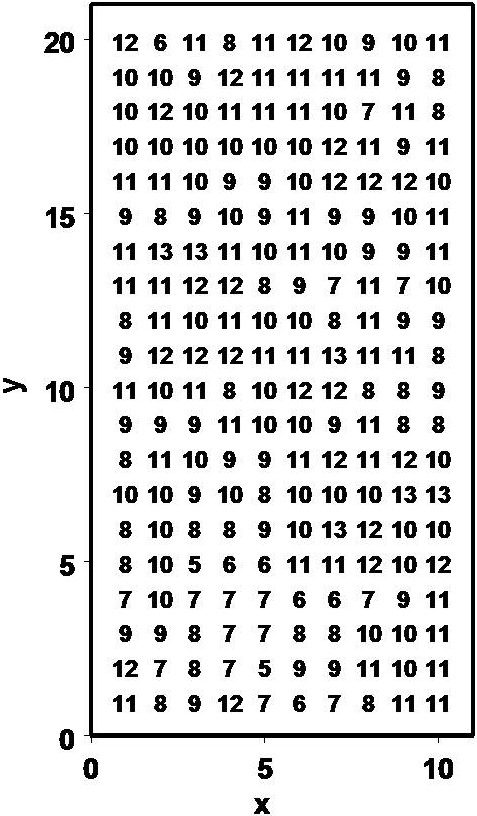
\includegraphics[width=\maxwidth]{figure/PlantSpGrid200-plot.jpg} &

		\vspace{2cm}
		\begin{tabular}{c}
		\cbl{1000 samplings} \\
		$\cbl{N = 200}$ \\ $\cbl{n = 100}$
		\end{tabular}

	\end{tabular}

\end{frame}

%-------------------------------------------------------------------------------
%                 Simulations
%-------------------------------------------------------------------------------

\begin{frame}[fragile]
\frametitle{Fixed Pattern, Random Samples}

1000 random samples of size 100 \\
\tiny
Ver Hoef, J.M.  2002.  Sampling and geostatistics for spatial data.  {\it Ecoscience} {\bf 9}: 152 - 161.\\
\footnotesize
	\begin{table}[ht]
	\centering
	\begin{tabular}{ccc}
	Validation Statistics & Simple Random Sample & Finite Block Pred \\ 
	\cbl{Bias} & \cre{-0.002} & \cre{-0.001} \\ 
	\cbl{RMSPE} & \cre{0.121} & \cre{0.106} \\ 
	\cbl{RAEV} & \cre{0.122} & \cre{0.105} \\ 
	\cbl{80\%CI} & \cre{0.802} & \cre{0.806} \\ 
	\end{tabular}
	\end{table}

\end{frame}

%-------------------------------------------------------------------------------
%                 Simulations
%-------------------------------------------------------------------------------

\begin{frame}[fragile]
\frametitle{Random Pattern, Fixed Samples}
\tiny
Ver Hoef, J.M.  2002.  Sampling and geostatistics for spatial data.  {\it Ecoscience} {\bf 9}: 152 - 161.\\
\vspace{.1cm}
	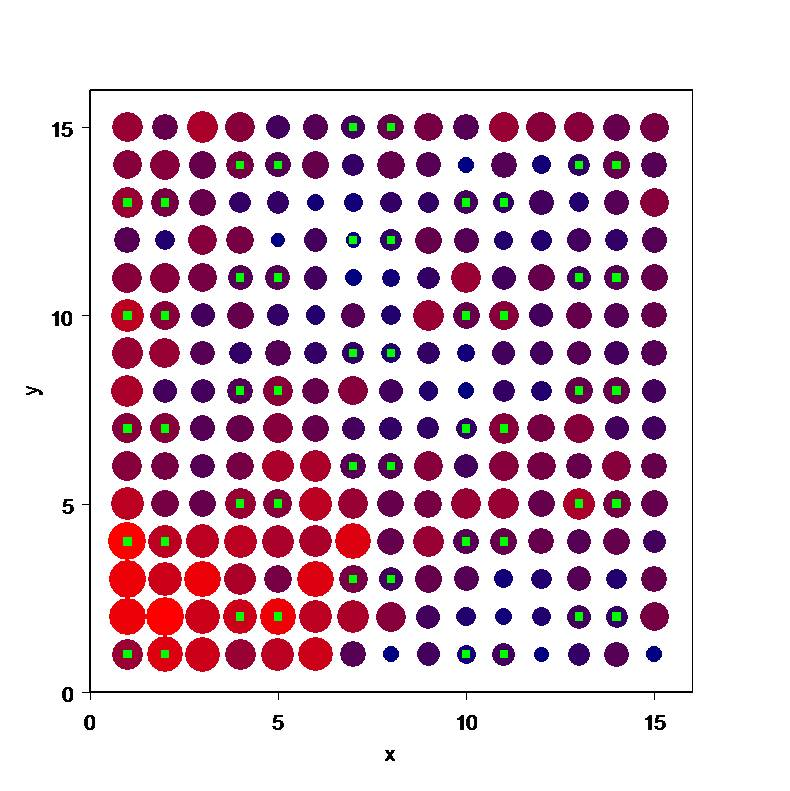
\includegraphics[width=.5\maxwidth]{figure/RandPatFixSamp1.jpg}
	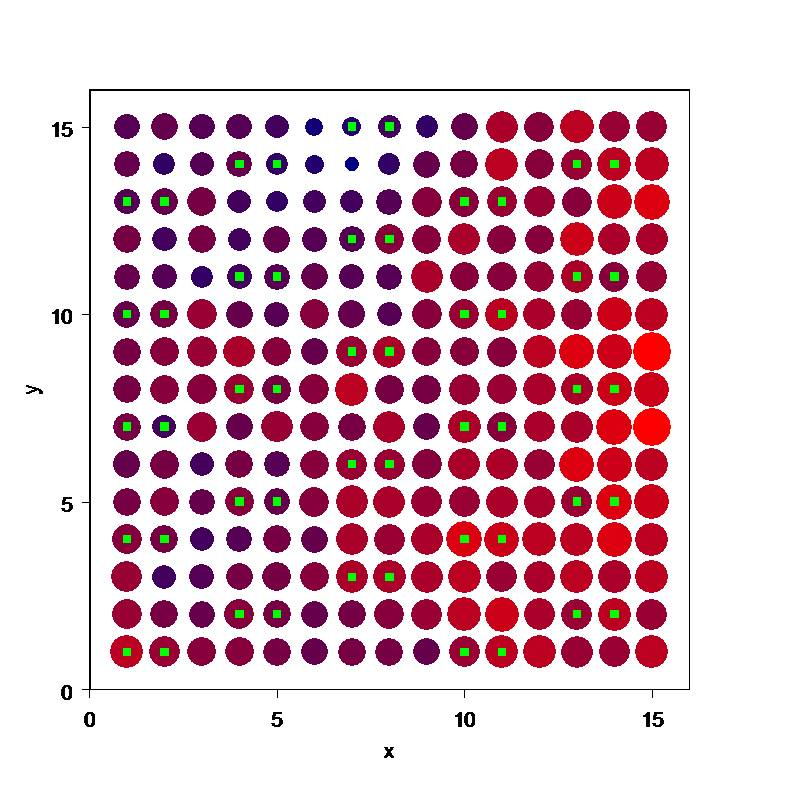
\includegraphics[width=.5\maxwidth]{figure/RandPatFixSamp2.jpg}

\end{frame}

%-------------------------------------------------------------------------------
%                 Simulations
%-------------------------------------------------------------------------------

\begin{frame}[fragile]
\frametitle{Random Pattern, Fixed Samples}

\footnotesize
	\begin{table}[ht]
	\centering
	\begin{tabular}{cccc}
	Validation Statistics & SRS$_{random}$ & FPBK$_{random}$ & FPBK$_{fixed}$\\ 
	\cbl{Bias} & \cre{0.522} & \cre{-0.181} & \cre{0.127} \\ 
	\cbl{RMSPE} & \cre{28.0} & \cre{20.7} & \cre{17.3} \\ 
	\cbl{RAEV} & \cre{28.0} & \cre{20.3} & \cre{17.5} \\ 
	\cbl{80\%CI} & \cre{0.801} & \cre{0.791} & \cre{0.796}\\ 
	\end{tabular}
	\end{table}

\end{frame}

%-------------------------------------------------------------------------------
%                 Simulations
%-------------------------------------------------------------------------------

\subsection{PLoS ONE paper 2013}
\begin{frame}[fragile]
\frametitle{Simulation With Covariates}

\footnotesize
Ver Hoef, J.M.  and Temesgen, H.  2013. A comparsion of the spatial linear model to nearest neighbor (k-NN) methods for forestry applications.  {\it PloS ONE} {\bf 8(3)}: e59129. doi:10.1371/journal.pone.0059129.

\begin{table}
\centering
$
\begin{array}{c}
	\bw_1 = \bz_1 + \bepsilon_1 \\
	\bw_\eta = \phi_{\eta-1}\bw_{\eta-1} + \bz_\eta + \bepsilon_\eta \\
	\bx_\eta = \bmu_\eta + \bw_\eta \\
	\by = \bX\bbeta + \bz_y + \bepsilon_y \\
\end{array}
$
\end{table}
\begin{center}
$	\bV[j,j\upp;\sigma^2,\rho] =  
		\sigma^2\left(1-\frac{3}{2}\frac{d_{j,j\upp}}{\rho}+
		\frac{1}{2}\frac{d_{j,j\upp}}{\rho^3}\right)
		    I\left(\frac{d_{j,j\upp}}{\rho}\leq 1\right) 
$
\end{center}

8 spatially-patterned and cross-correlated covariates \\
2 excluded, 2 with $\beta_i = 0$ included

\end{frame}

%-------------------------------------------------------------------------------
%                 Prediction Methods
%-------------------------------------------------------------------------------
\begin{frame}[fragile]
\frametitle{Prediction Methods}

\footnotesize
\begin{itemize}
\item mah1 k-NN that uses Mahalanobis distance with $k=1$.
\item mah5: k-NN that uses Mahalanobis distance with $k=5$.
\item msn1: k-NN that uses most significant neighbor (MSN) with $k=1$.
\item msn5: k-NN that uses MSN with $k=1$.
\item best: k-NN that uses both Mahalanobis distance and MSN, and tries $k=1, 2, \ldots, 30$, and then chooses the distance matrix and $k$ with the smallest cross-validation RMSPE from the observed data.
\item slm: a spatial linear model using the same covariates as all k-NN methods as main effects only, with an exponential autocovariance model estimated by REML, and using FPBK prediction and variance equations.
\item lm: multiple regression like slmMain but assuming all random errors are independent.
\end{itemize}

\end{frame}

%-------------------------------------------------------------------------------
%                 Simulations
%-------------------------------------------------------------------------------
\begin{frame}[fragile]
\frametitle{Performance Measures}
\tiny
\begin{itemize}
	\item 
	Root-mean-squared-prediction error (RMSPE): 
	\[
		\textrm{RMSPE}=\sqrt{\frac{1}{m}\sum_{j=1}^m(\hat{\theta}_j-\theta_j)^2},
	\]

	\item
		SRB: signed relative bias.
	\[
		\textrm{SRB}=\textrm{sign}(\tau)\sqrt{\frac{\tau^2}{\textrm{MSPE}-\tau^2}},
	\]
	where
	\[
		\tau=\frac{1}{m}\sum_{j=1}^m(\hat{\theta}_j-\theta_j),
	\]
	and sign($\tau$) is the sign (positive or negative) of $\tau$.
	\item
	PIC90: 90\% prediction interval coverage
	\[
		\textrm{PIC90}=\frac{1}{m}\sum_{j=1}^mI\left(\left(\hat{\theta}_j-1.645\hat{\textrm{se}}(\hat{\theta}_j)\right) < \theta_j \; \& \;  \theta_j < \left(\hat{\theta}_j+1.645\hat{\textrm{se}}(\hat{\theta}_j)\right) \right),
	\]
where 
$\hat{\textrm{se}}(\hat{\theta}_j)$ is the estimated standard error of  $\hat{\theta}_j$. 
\end{itemize}

\end{frame}

%-------------------------------------------------------------------------------
%                 Simulations
%-------------------------------------------------------------------------------
\begin{frame}[fragile]
\frametitle{Gaussian Simulations}


\begin{table}[ht]
\caption{\tiny Performance summaries from 2000 simulated spatial Gaussian data sets with 100 samples and 300 predictions each. Prediction methods form the columns and are described in Section 3.4.  Performance measures form the rows and are described in Section 3.3. \label{GAUSsummary}}
\scriptsize
\begin{center}
\begin{tabular}{|l r r r r r r r|}
\hline
\hline
  & mah1 & mah5 & msn1 & msn5 & best & lm & slm \\
\hline
\hline
\multicolumn{8}{|c|}{Point} \\
RMSPE$^a$ & 9.329 & 7.451 & 5.379 & 4.423 & 4.456 & 3.892 & 2.443 \\
SRB$^b$ & -0.006 & -0.009 & 0 & -0.004 & -0.004 & -0.002 & 0.001 \\
PIC90$^c$ & 0.897 & 0.9 & 0.887 & 0.889 & 0.88 & 0.896 & 0.892 \\
\multicolumn{8}{|c|}{Total} \\
RMSPE & 262.6 & 289.8 & 174.3 & 153.3 & 154.5 & 139.3 & 87.8 \\
SRB & -0.058 & -0.067 & -0.003 & -0.034 & -0.034 & -0.02 & 0.009 \\
PIC90 & 0.952 & 0.87 & 0.914 & 0.886 & 0.874 & 0.88 & 0.887 \\
\hline
\multicolumn{8}{l}{$^a$ Root-mean-squared-prediction error} \\
\multicolumn{8}{l}{$^b$ Signed relative bias} \\
\multicolumn{8}{l}{$^c$ 90\% prediction interval coverage} \\
\end{tabular}
\end{center}
\end{table}%
%
\end{frame}

%-------------------------------------------------------------------------------
%                 Simulations
%-------------------------------------------------------------------------------
\begin{frame}[fragile]
\frametitle{Poisson Simulations}


\begin{table}[ht]
\caption{\tiny Performance summaries from 2000 simulated Poisson data sets with 100 samples and 300 predictions each. Prediction methods form the columns and are described in Section 3.4.  Performance measures form the rows and are described in Section 3.3. \label{POISsummary}}
\scriptsize
\begin{center}
\begin{tabular}{|l r r r r r r r|}
\hline
\hline
  & mah1 & mah5 & msn1 & msn5 & best & lm & slm \\
\hline
\hline
\multicolumn{8}{|c|}{Total} \\
RMSPE & 320 & 295.9 & 296.3 & 262.3 & 272.2 & 283.1 & 226.1 \\
SRB & -0.137 & -0.188 & -0.047 & -0.135 & -0.182 & -0.033 & -0.005 \\
PIC90 & 0.912 & 0.842 & 0.9 & 0.867 & 0.83 & 0.86 & 0.858 \\
\hline
\end{tabular}
\end{center}
\end{table}%

\end{frame}

%-------------------------------------------------------------------------------
%                 Simulations
%-------------------------------------------------------------------------------
\begin{frame}[fragile]
\frametitle{Bernoulli Simulations}


\begin{table}[ht]
\caption{\tiny Performance summaries from 2000 simulated binary data sets with 100 samples and 300 predictions each. Prediction methods form the columns and are described in Section 3.4.  Performance measures form the rows and are described in Section 3.3. \label{BERNsummary}}
\scriptsize
\begin{center}
\begin{tabular}{|l r r r r r r r|}
\hline
\hline
  & mah1 & mah5 & msn1 & msn5 & best & lm & slm \\
\hline
\hline
\multicolumn{8}{|c|}{Proportion} \\
RMSPE & 0.0395 & 0.0394 & 0.0387 & 0.0334 & 0.0343 & 0.0329 & 0.0298 \\
SRB & 0.072 & 0.09 & 0.003 & 0.019 & 0.079 & 0.018 & 0.014 \\
PIC90 & 0.919 & 0.841 & 0.913 & 0.882 & 0.84 & 0.886 & 0.884 \\
\hline
\end{tabular}
\end{center}
\end{table}%
%

\end{frame}


%-------------------------------------------------------------------------------
%                 Simulations
%-------------------------------------------------------------------------------

\begin{frame}[fragile]
\frametitle{Forestry Data Resampling PMAI}

	\begin{tabular}	{p{5cm} p{4cm}}
		\vspace{-.1cm}
		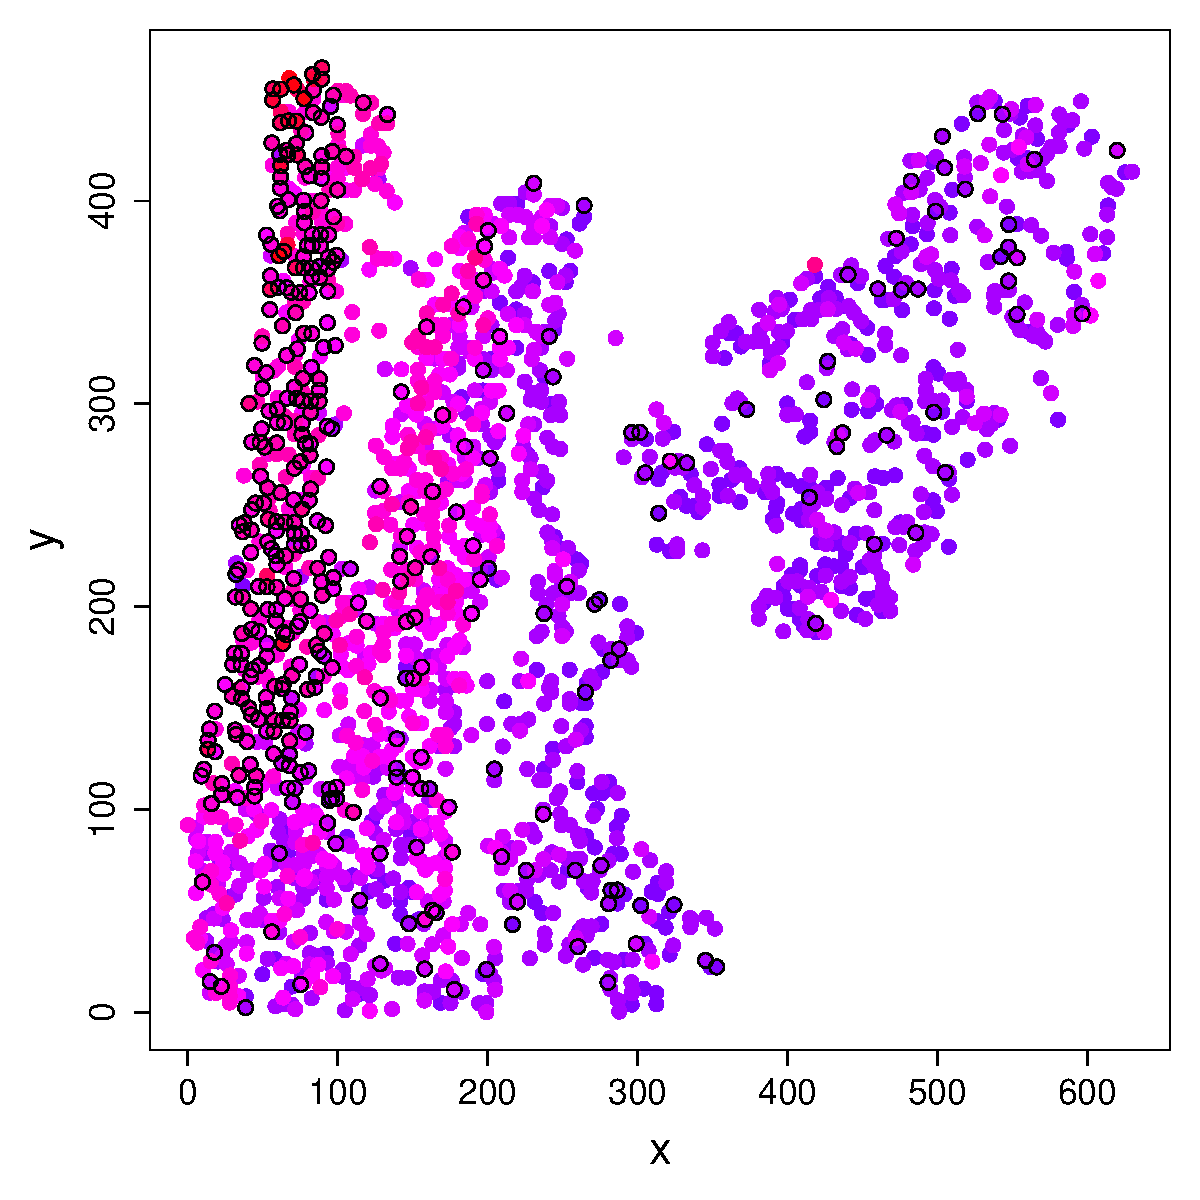
\includegraphics[width=\maxwidth]{figure/pmaiUnbalSamp} &
		\vspace{-.1cm}
		\footnotesize
		\begin{itemize}
			\item response: maximum potential mean annual increment (PMAI)
			\item covariates: 1) temperature, 2) precipitation, 3)Climate Moisture Index, 4) an indicator variable for shade tolerance based on Western Hemlock trees, and 5) elevation
		\end{itemize}
	\end{tabular}

\end{frame}

%-------------------------------------------------------------------------------
%                 Simulations
%-------------------------------------------------------------------------------

\begin{frame}[fragile]
\frametitle{PMAI Resampling}

\begin{table}[ht]
\caption{\tiny Performance summaries for 500 resamplings of PMAI forest data with 386 samples and 1500 predictions each. Prediction methods form the columns and are described in Section 3.4.  Performance measures form the rows and are described in Section 3.3. \label{PMAIsummary}}
\scriptsize
\begin{center}
\begin{tabular}{|l r r r r r r r|}
\hline
\hline
  & mah1 & mah5 & msn1 & msn5 & best & lm & slm \\
\hline
\hline
\multicolumn{8}{|c|}{Total} \\
RMSPE & 219.1 & 230.7 & 243.3 & 200.9 & 223.2 & 197 & 180.4 \\
SRB & 0.437 & 0.712 & 0.064 & -0.019 & 0.446 & 0.082 & 0.058 \\
PIC90 & 0.944 & 0.838 & 0.948 & 0.922 & 0.834 & 0.904 & 0.904 \\
\hline
\end{tabular}
\end{center}
\end{table}%

\end{frame}

%-------------------------------------------------------------------------------
%                 Simulations
%-------------------------------------------------------------------------------

\begin{frame}[fragile]
\frametitle{PMAI Resampling with Unbalanced Sampling}

\begin{table}[ht]
\caption{\tiny Performance summaries for 500 resamplings of PMAI forest data with 386 spatially unbalanced samples and 1500 predictions each. \label{PREFsummary}}
\scriptsize
\begin{center}
\begin{tabular}{|l r r r r r r r|}
\hline
\hline
  & mah1 & mah5 & msn1 & msn5 & best & lm & slm \\
\hline
\hline
\multicolumn{8}{|c|}{Total} \\
RMSPE & 637.9 & 853.6 & 457.1 & 442.2 & 576.1 & 608.1 & 269 \\
SRB & 2.635 & 4.055 & 1.418 & 1.77 & 1.651 & 2.86 & 0.369 \\
PIC90 & 0.248 & 0.010 & 0.626 & 0.438 & 0.308 & 0.128 & 0.92 \\
\hline
\end{tabular}
\end{center}
\end{table}%
%

\end{frame}

%-------------------------------------------------------------------------------
%                 Examples
%-------------------------------------------------------------------------------

\section{Examples}
\subsection{}
\begin{frame}[fragile]
\frametitle{Nome Moose Survey}













	\vspace{-.1cm}
	\begin{tabular}{c}
			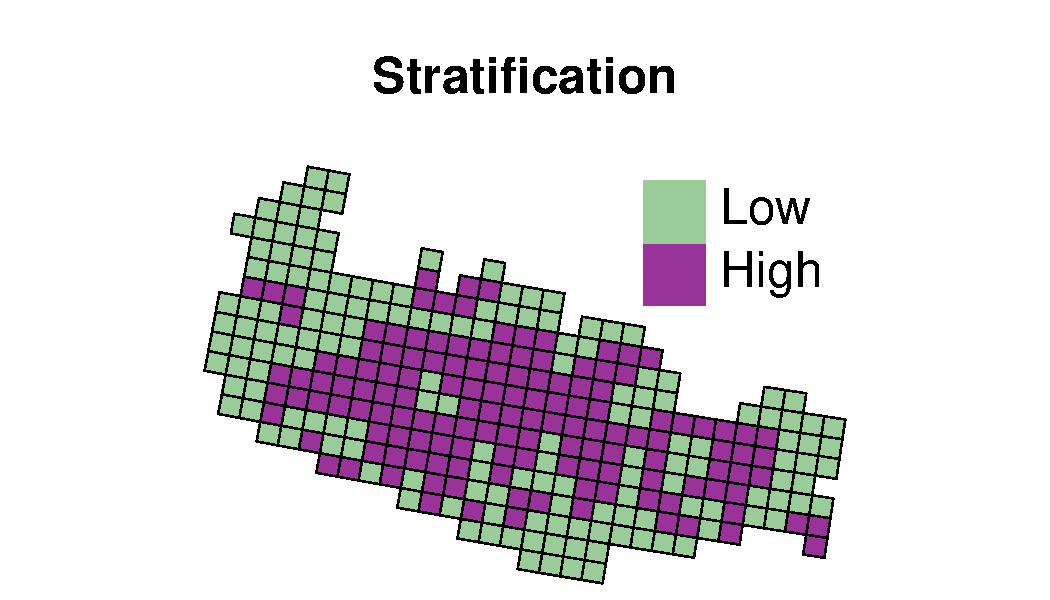
\includegraphics[width=.5\maxwidth]{figure/mooseStrat-plot} 
			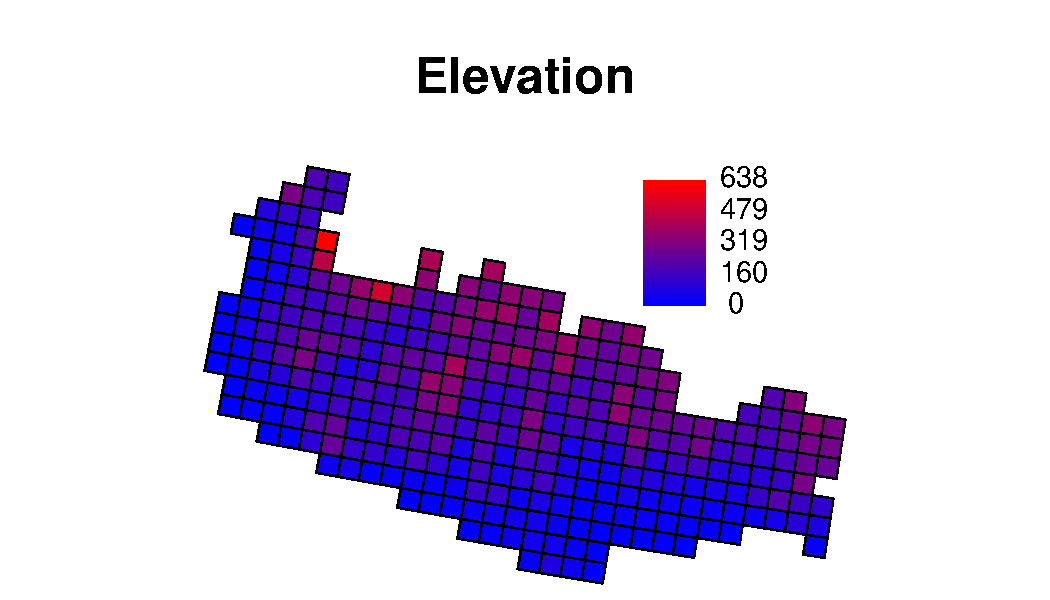
\includegraphics[width=.5\maxwidth]{figure/mooseElev-plot} \\
			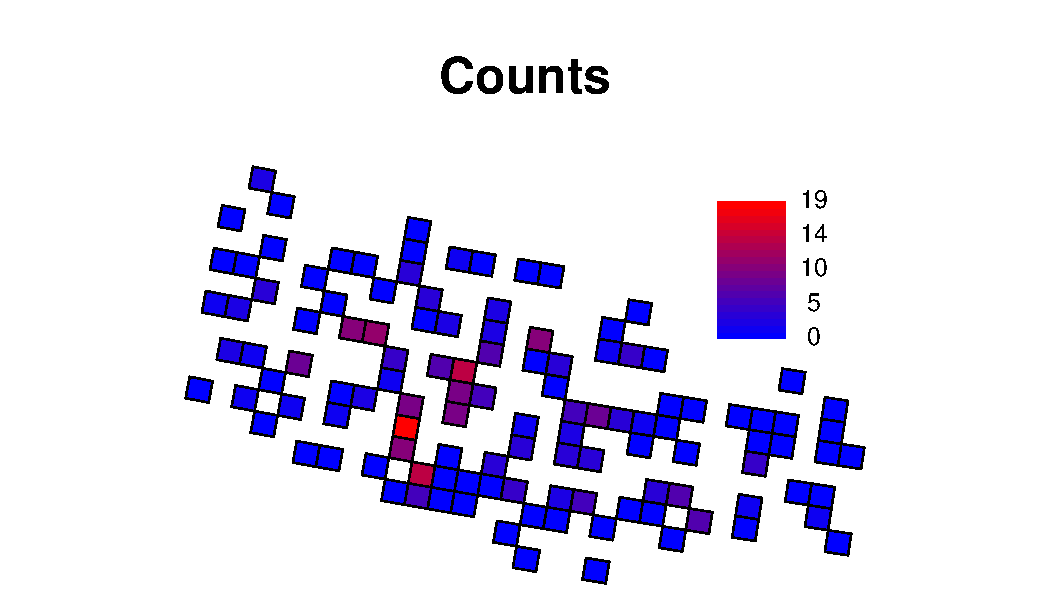
\includegraphics[width=.6\maxwidth]{figure/mooseCounts-plot} 
	\end{tabular}

\end{frame}

%-------------------------------------------------------------------------------
%                 Examples
%-------------------------------------------------------------------------------

\begin{frame}[fragile]
\frametitle{Nome Moose Survey}

\begin{knitrout}\tiny
\definecolor{shadecolor}{rgb}{0.969, 0.969, 0.969}\color{fgcolor}\begin{kframe}
\begin{alltt}
\hlfunctioncall{library}(spPlotSampCourse)
\hlfunctioncall{library}(maptools)
path <- \hlfunctioncall{system.file}(\hlstring{"rawdata/moose"}, package = \hlstring{"spPlotSampCourse"})
samplesFile <- \hlfunctioncall{paste}(path, \hlstring{"/"}, \hlstring{"Samples"}, sep = \hlstring{""})
samples <- \hlfunctioncall{readShapePoly}(samplesFile)
samples@data[, \hlstring{"x"}] <- \hlfunctioncall{LLtoUTM}(samples@data[, \hlstring{"CENTRLAT"}], samples@data[, \hlstring{"CENTRLON"}])[, 
    \hlstring{"x"}]
samples@data[, \hlstring{"y"}] <- \hlfunctioncall{LLtoUTM}(samples@data[, \hlstring{"CENTRLAT"}], samples@data[, \hlstring{"CENTRLON"}])[, 
    \hlstring{"y"}]
samples@data[, \hlstring{"TOTAL"}] <- \hlfunctioncall{as.numeric}(\hlfunctioncall{as.character}(samples@data[, \hlstring{"TOTAL"}]))
samples@data[, \hlstring{"b"}] <- \hlfunctioncall{rep}(1, times = \hlfunctioncall{length}(samples@data[, 1]))
sdata <- samples@data
\hlfunctioncall{coordinates}(sdata) <- \hlfunctioncall{c}(\hlstring{"x"}, \hlstring{"y"})
\end{alltt}
\end{kframe}
\end{knitrout}


\end{frame}

%-------------------------------------------------------------------------------
%                 Examples
%-------------------------------------------------------------------------------

\begin{frame}[fragile]
\frametitle{Nome Moose Survey}

\begin{knitrout}\tiny
\definecolor{shadecolor}{rgb}{0.969, 0.969, 0.969}\color{fgcolor}\begin{kframe}
\begin{alltt}
moFit <- \hlfunctioncall{splmm}(TOTAL ~ ELEVMEAN + STRAT, spdata = sdata, varComps = \hlstring{"exponential"})
\hlcomment{# summary(moFit)}
\hlfunctioncall{summary}(moFit)$coefficients
\end{alltt}
\begin{verbatim}
##              Estimate Std. Error t value  Pr(>|t|)
## (Intercept)  2.592622   0.711248  3.6452 0.0004013
## ELEVMEAN     0.001019   0.003291  0.3097 0.7573331
## STRATL      -2.232373   0.611141 -3.6528 0.0003908
\end{verbatim}
\begin{alltt}
\hlfunctioncall{summary}(moFit)$covparms
\end{alltt}
\begin{verbatim}
##   Variance Component Parameter Type  Estimate
## 1             nugget         nugget 1.928e-05
## 2        exponential         parsil 1.006e+01
## 3        exponential          range 1.043e+01
\end{verbatim}
\end{kframe}
\end{knitrout}


\end{frame}

%-------------------------------------------------------------------------------
%                 Examples
%-------------------------------------------------------------------------------
\begin{frame}[fragile]
\frametitle{Nome Moose Survey}

\begin{knitrout}\tiny
\definecolor{shadecolor}{rgb}{0.969, 0.969, 0.969}\color{fgcolor}\begin{kframe}
\begin{alltt}
moFit <- \hlfunctioncall{splmm}(TOTAL ~ STRAT - 1, spdata = sdata, varComps = \hlstring{"exponential"})
\hlfunctioncall{summary}(moFit)$coefficients
\end{alltt}
\begin{verbatim}
##        Estimate Std. Error t value  Pr(>|t|)
## STRATH   2.7442     0.5429  5.0547 1.609e-06
## STRATL   0.5289     0.5725  0.9239 3.574e-01
\end{verbatim}
\begin{alltt}
\hlfunctioncall{summary}(moFit)$covparms
\end{alltt}
\begin{verbatim}
##   Variance Component Parameter Type  Estimate
## 1             nugget         nugget 1.287e-04
## 2        exponential         parsil 9.925e+00
## 3        exponential          range 1.023e+01
\end{verbatim}
\begin{alltt}
FPBK <- \hlfunctioncall{predictBlockFinPop}(moFit, \hlstring{"b"})
FPBK
\end{alltt}
\begin{verbatim}
##    Resp Wts  Pred Pred SE
## 1 TOTAL   b 554.6   60.62
\end{verbatim}
\end{kframe}
\end{knitrout}


\end{frame}

%-------------------------------------------------------------------------------
%                 Examples
%-------------------------------------------------------------------------------
\begin{frame}[fragile]
\frametitle{Nome Moose Survey}

\begin{knitrout}\tiny
\definecolor{shadecolor}{rgb}{0.969, 0.969, 0.969}\color{fgcolor}\begin{kframe}
\begin{alltt}
samples.H <- samples[samples@data[, \hlstring{"STRAT"}] == \hlstring{"H"}, ]
samples.L <- samples[samples@data[, \hlstring{"STRAT"}] == \hlstring{"L"}, ]
sdataH <- samples.H@data
\hlfunctioncall{coordinates}(sdataH) <- \hlfunctioncall{c}(\hlstring{"x"}, \hlstring{"y"})
sdataL <- samples.L@data
\hlfunctioncall{coordinates}(sdataL) <- \hlfunctioncall{c}(\hlstring{"x"}, \hlstring{"y"})
moFitH <- \hlfunctioncall{splmm}(TOTAL ~ 1, spdata = sdataH, varComps = \hlstring{"exponential"})
\hlfunctioncall{summary}(moFitH)$coefficients
\end{alltt}
\begin{verbatim}
##             Estimate Std. Error t value  Pr(>|t|)
## (Intercept)     2.78     0.7452   3.731 0.0003782
\end{verbatim}
\begin{alltt}
moFitL <- \hlfunctioncall{splmm}(TOTAL ~ 1, spdata = sdataL, varComps = \hlstring{"exponential"})
\hlfunctioncall{summary}(moFitL)$coefficients
\end{alltt}
\begin{verbatim}
##             Estimate Std. Error  t value Pr(>|t|)
## (Intercept)   0.3082      45.94 0.006709   0.9947
\end{verbatim}
\end{kframe}
\end{knitrout}


\end{frame}

%-------------------------------------------------------------------------------
%                 Examples
%-------------------------------------------------------------------------------
\begin{frame}[fragile]
\frametitle{Nome Moose Survey}

\begin{knitrout}\tiny
\definecolor{shadecolor}{rgb}{0.969, 0.969, 0.969}\color{fgcolor}\begin{kframe}
\begin{alltt}
FPBK.H <- \hlfunctioncall{predictBlockFinPop}(moFitH, \hlstring{"b"})
FPBK.L <- \hlfunctioncall{predictBlockFinPop}(moFitL, \hlstring{"b"})
\hlfunctioncall{rbind}(FPBK.H, FPBK.L)
\end{alltt}
\begin{verbatim}
##    Resp Wts   Pred Pred SE
## 1 TOTAL   b 501.26   38.40
## 2 TOTAL   b  51.38   14.08
\end{verbatim}
\begin{alltt}
FPBK.strat <- \hlfunctioncall{data.frame}(Pred = FPBK.H[, \hlstring{"Pred"}] + FPBK.L[, \hlstring{"Pred"}], PredSE = \hlfunctioncall{sqrt}(FPBK.H[, 
    \hlstring{"Pred SE"}]^2 + FPBK.L[, \hlstring{"Pred SE"}]^2))
FPBK.strat
\end{alltt}
\begin{verbatim}
##    Pred PredSE
## 1 552.6   40.9
\end{verbatim}
\begin{alltt}
FPBK
\end{alltt}
\begin{verbatim}
##    Resp Wts  Pred Pred SE
## 1 TOTAL   b 554.6   60.62
\end{verbatim}
\end{kframe}
\end{knitrout}


\end{frame}

%-------------------------------------------------------------------------------
%                 Robustness
%-------------------------------------------------------------------------------
\section{Robustness}
\subsection{}
\begin{frame}[fragile]
\frametitle{Robustness of Block Prediction Methods}

\begin{itemize}
	\item BLUP is non-parametric
	\item REML are estimating equations, so covariance estimation is non-parametric
	\item Predictions are robust to mis-specification of covariance model
	\item Both predictor and predictand are linear combinations, so we can appeal to a correlated version of central limit theorem and use normal-distribution for probability statements (e.g., prediction intervals).
\end{itemize}

\end{frame}

\end{document}
